\documentclass[11pt]{article}

\usepackage[utf8]{inputenc}
\usepackage[T1]{fontenc}
\usepackage{lmodern}
\usepackage[margin=1in]{geometry}
\usepackage{setspace}
\usepackage{booktabs}
\usepackage{longtable}
\usepackage{array}
\usepackage{enumitem}
\usepackage{amsmath}
\usepackage{hyperref}
\usepackage{xcolor}
\usepackage{graphicx}
\usepackage{float}

\hypersetup{
    colorlinks=true,
    linkcolor=blue,
    urlcolor=blue,
    pdftitle={Week 5 - Representation and Dimensionality Report},
    pdfauthor={MovieLens Discovery Project Team}
}

\setstretch{1.08}
\setlength{\parskip}{0.5em}
\setlength{\parindent}{0pt}

\title{Week 5 - Representation and Dimensionality Report}
\date{April 2026}

\begin{document}

\maketitle

\section{Executive Summary}

This report documents the feature engineering and dimensionality reduction analysis for the MovieLens 25M project. We built a consolidated movie-level feature matrix (62,423 movies \(\times\) 45 features) and applied PCA to quantify structure and compression potential.

\textbf{Key findings}

\begin{itemize}[leftmargin=1.5em]
    \item The MovieLens dataset is multidimensional: the first two principal components capture only 12.90\% of variance.
    \item 30 components retain 80.96\% of variance, a 66\% size reduction.
    \item PC1 captures popularity and richness; PC2 separates genre tone.
    \item Redundant features were removed while preserving a stable 45-feature set.
\end{itemize}

\textbf{Project context}

\begin{itemize}[leftmargin=1.5em]
    \item \textbf{Project title}: Personalized Movie Discovery and Recommendation Engine (MovieLens 25M)
    \item \textbf{Dataset}: MovieLens 25M (62,423 movies, 25M ratings, 1.09M tags)
    \item \textbf{Week 5 objective}: Build a representation layer and study dimensionality reduction
    \item \textbf{Status}: Complete, all artifacts generated and validated
\end{itemize}

\section{Why This Step Exists}

Week 3 established the cleaned data layer. Week 5 converts those tables into a numerical representation that can support clustering, recommendation, and graph work. The goal is to quantify how much of the movie structure can be captured in a compact latent space.

This matters because it:

\begin{enumerate}[leftmargin=1.5em]
    \item Reveals redundancy in engineered features.
    \item Shows which signals dominate (popularity, genre, era, tags).
    \item Produces a compact input space for Week 7 clustering.
\end{enumerate}

\section{Feature Engineering}

We built a consolidated, movie-level feature matrix from the Week 3 processed dataset. The final matrix contains \textbf{45 features} across three blocks.

\subsection{Feature blocks (final)}

\textbf{Numeric features (6)}

\begin{itemize}[leftmargin=1.5em]
    \item \texttt{release\_year\_z}
    \item \texttt{avg\_rating\_z}
    \item \texttt{rating\_std}
    \item \texttt{rating\_count\_log}
    \item \texttt{unique\_tag\_count\_log}
    \item \texttt{genre\_count\_log}
\end{itemize}

\textbf{Genre indicators (19)}

\begin{itemize}[leftmargin=1.5em]
    \item Binary features for the top 20 genres (19 present)
\end{itemize}

\textbf{Tag indicators (20)}

\begin{itemize}[leftmargin=1.5em]
    \item Binary features for the top 20 tags by frequency
\end{itemize}

\subsection{Normalization strategy}

\begin{itemize}[leftmargin=1.5em]
    \item Log1p normalization applied to count features
    \item Z-score normalization applied to release year and average rating
    \item Binary encoding for top genres and tags
    \item Min-max scaling not used; z-score preserves variance for PCA
\end{itemize}

\subsection{Feature redundancy validation}

During feature engineering, we identified and removed three highly correlated features:

\begin{enumerate}[leftmargin=1.5em]
    \item \textbf{tag\_event\_count\_log}: Pearson r=0.985 with unique\_tag\_count\_log
    \item \textbf{rating\_span\_seconds\_z}: implicit in rating\_count
    \item \textbf{tag\_span\_seconds\_z}: implicit in tag event counts
\end{enumerate}

\textbf{Validation of remaining features}

\begin{itemize}[leftmargin=1.5em]
    \item Pearson r=0.292 between genre\_count\_log and unique\_tag\_count\_log
    \item Both retained as independent signals
\end{itemize}

\subsection{Feature consistency checks}

\begin{itemize}[leftmargin=1.5em]
    \item Movies with ratings: 59,047
    \item Movies with tags: 45,251
    \item Movies with genres: 57,361
\end{itemize}

\subsection{Data sources}

\begin{itemize}[leftmargin=1.5em]
    \item \texttt{data/processed/week03\_v1/movies\_catalog.parquet}
    \item \texttt{data/processed/week03\_v1/movie\_genres.parquet}
    \item \texttt{data/processed/week03\_v1/ratings\_clean.parquet}
    \item \texttt{data/processed/week03\_v1/tags\_clean.parquet}
\end{itemize}

\section{PCA Results and Variance Analysis}

We applied PCA (via SVD) to the standardized 62,423 \(\times\) 45 feature matrix.

\subsection{Explained variance structure}

\begin{table}[H]
\centering
\begin{tabular}{lcc}
\toprule
Component & Explained Variance & Cumulative Variance \\
\midrule
PC1 & 0.0802 & 0.0802 \\
PC2 & 0.0488 & 0.1290 \\
PC3 & 0.0447 & 0.1737 \\
PC4 & 0.0418 & 0.2155 \\
PC5 & 0.0344 & 0.2498 \\
\bottomrule
\end{tabular}
\caption{Explained variance ratios for the first five components.}
\end{table}

Individual components contribute 3--8\% each. No single factor dominates; variance spreads across independent dimensions such as popularity, genre tone, release era, rating consensus, and tagging intensity.

\subsection{Compression milestones}

\begin{table}[H]
\centering
\begin{tabular}{lc}
\toprule
Components & Cumulative Variance \\
\midrule
30 & 0.8096 \\
36 & 0.9058 \\
40 & 0.9609 \\
\bottomrule
\end{tabular}
\caption{Variance retention thresholds from \texttt{week05\_pca\_thresholds.csv}.}
\end{table}

Use 30 components for clustering and recommendation: it retains more than 80\% of variance while cutting the feature count by two-thirds.

\subsection{Reconstruction error}

\begin{table}[H]
\centering
\begin{tabular}{lccc}
\toprule
Components & Retained Variance & MSE & Relative Frobenius Error \\
\midrule
10 & 0.3998 & 0.6002 & 0.7747 \\
20 & 0.6237 & 0.3763 & 0.6134 \\
30 & 0.8096 & 0.1904 & 0.4364 \\
36 & 0.9058 & 0.0942 & 0.3069 \\
40 & 0.9609 & 0.0391 & 0.1976 \\
\bottomrule
\end{tabular}
\caption{Reconstruction error summary from \texttt{week05\_reconstruction\_error.csv}.}
\end{table}

At 30 components, MSE = 0.1904, which is an acceptable trade-off between compression and fidelity.

\section{Principal Component Interpretation}

\subsection{PC1: Movie Richness and Popularity}

\begin{table}[H]
\centering
\begin{tabular}{lc}
\toprule
Feature & Loading \\
\midrule
rating\_count\_log & -0.429 \\
unique\_tag\_count\_log & -0.413 \\
genre\_count\_log & -0.313 \\
rating\_std & -0.198 \\
tag\_019\_action & -0.187 \\
\bottomrule
\end{tabular}
\caption{Top PC1 loadings from \texttt{week05\_pca\_top\_loadings.csv}.}
\end{table}

PC1 separates prominent, highly rated, richly tagged movies from niche or low-activity movies.

\subsection{PC2: Genre Profile}

\begin{table}[H]
\centering
\begin{tabular}{lc}
\toprule
Feature & Loading \\
\midrule
genre\_thriller & -0.407 \\
genre\_action & -0.277 \\
genre\_horror & -0.257 \\
genre\_crime & -0.256 \\
genre\_comedy & 0.243 \\
\bottomrule
\end{tabular}
\caption{Top PC2 loadings from \texttt{week05\_pca\_top\_loadings.csv}.}
\end{table}

PC2 contrasts intense genres (action, thriller, horror, crime) against lighter genres (comedy).

\subsection{Key takeaways}

Multiple independent dimensions drive movie differences. PC1 and PC2 align with intuitive movie properties, supporting interpretability and downstream clustering.

At 30 components, we keep about 81\% of the signal while losing mostly noise, which should help clustering. The remaining 45 features are orthogonal and well-separated, so downstream methods like matrix factorization should work well.

\section{Generated Artifacts (artifacts/week05)}

\subsection{Data files}

\begin{itemize}[leftmargin=1.5em]
    \item \texttt{week05\_movie\_feature\_frame.parquet}
    \item \texttt{week05\_pca\_feature\_matrix.parquet}
    \item \texttt{week05\_pca\_scores.parquet}
    \item \texttt{week05\_feature\_catalog.csv}
\end{itemize}

\subsection{Analysis tables}

\begin{itemize}[leftmargin=1.5em]
    \item \texttt{week05\_feature\_profile.csv}
    \item \texttt{week05\_sanity\_checks.csv}
    \item \texttt{week05\_pca\_summary.csv}
    \item \texttt{week05\_pca\_thresholds.csv}
    \item \texttt{week05\_reconstruction\_error.csv}
    \item \texttt{week05\_pca\_top\_loadings.csv}
\end{itemize}

\subsection{Visualizations}

\begin{itemize}[leftmargin=1.5em]
    \item \texttt{week05\_pca\_elbow\_rule.png}
    \item \texttt{week05\_pca\_explained\_variance.png}
    \item \texttt{week05\_pca\_scatter\_pc1\_pc2.png}
    \item \texttt{week05\_pca\_scatter\_pc1\_pc3.png}
    \item \texttt{week05\_pca\_biplot\_loadings.png}
\end{itemize}

\subsection{Embedded figures}

\begin{figure}[H]
\centering
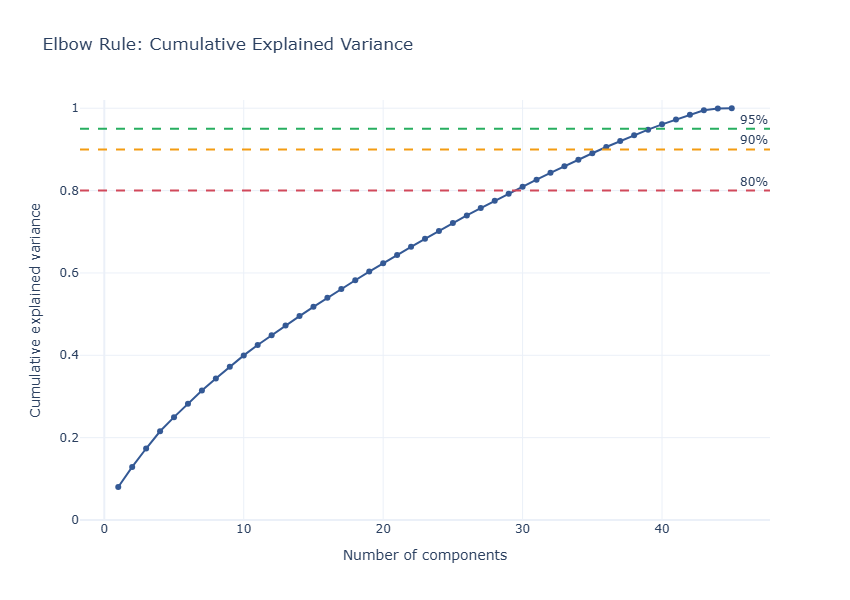
\includegraphics[width=0.85\textwidth]{../../artifacts/week05/week05_pca_elbow_rule.png}
\caption{Cumulative explained variance with 80/90/95\% thresholds.}
\end{figure}

\begin{figure}[H]
\centering
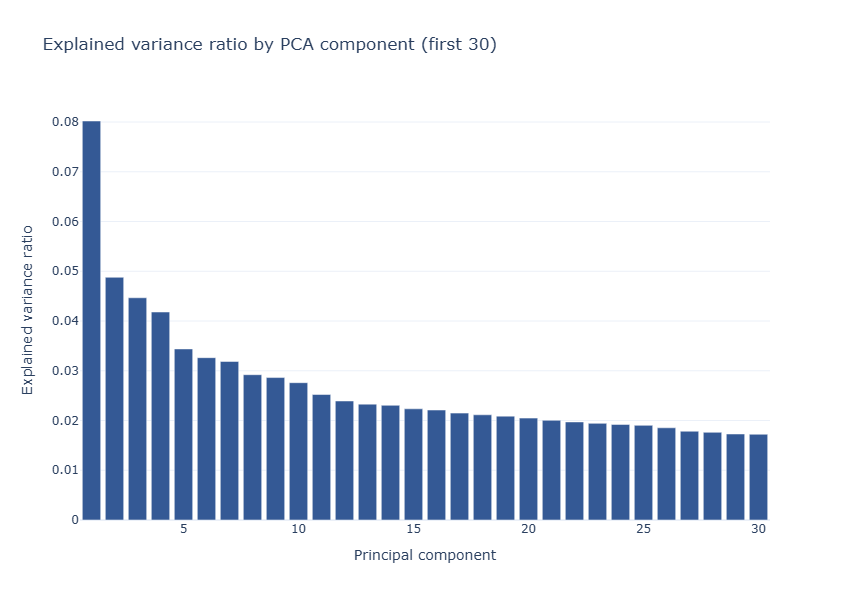
\includegraphics[width=0.85\textwidth]{../../artifacts/week05/week05_pca_explained_variance.png}
\caption{Explained variance for the first components.}
\end{figure}

\begin{figure}[H]
\centering
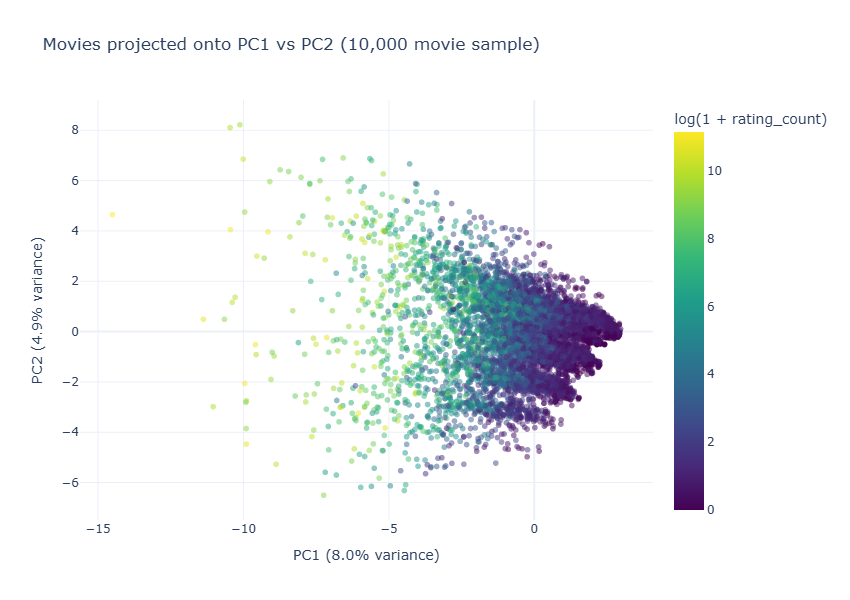
\includegraphics[width=0.85\textwidth]{../../artifacts/week05/week05_pca_scatter_pc1_pc2.png}
\caption{PCA scatter plot for PC1 vs. PC2.}
\end{figure}

\begin{figure}[H]
\centering
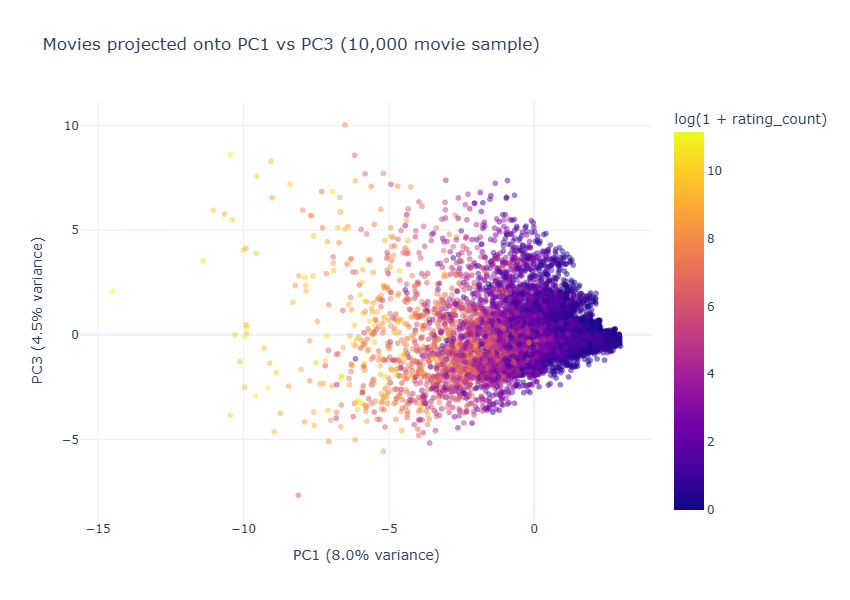
\includegraphics[width=0.85\textwidth]{../../artifacts/week05/week05_pca_scatter_pc1_pc3.png}
\caption{PCA scatter plot for PC1 vs. PC3.}
\end{figure}

\begin{figure}[H]
\centering
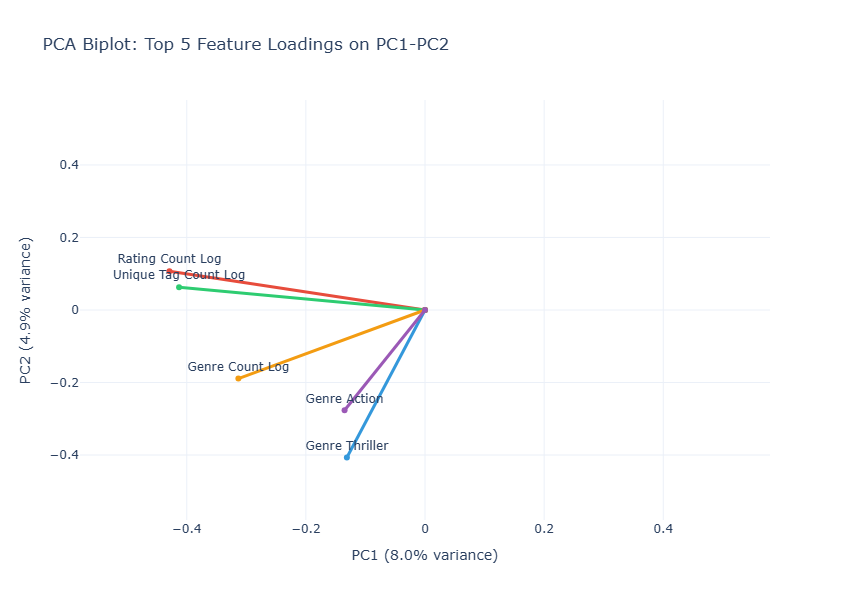
\includegraphics[width=0.85\textwidth]{../../artifacts/week05/week05_pca_biplot_loadings.png}
\caption{Biplot with top loading vectors.}
\end{figure}

\section{Interpretation and Implications}

\subsection{What the variance structure tells us}

No single dimension dominates. PC1 explains only 8\% of variance, which means movie differences cut across multiple independent axes: popularity, genre tone, release era, rating spread, and tagging intensity.

\subsection{Compression strategy for Week 7}

For clustering and recommendation, we recommend using the 30-component compressed space instead of the full 45 features.

\textbf{Benefits}

\begin{itemize}[leftmargin=1.5em]
    \item Keeps 80.96\% of variance
    \item Cuts feature count by 66\%
    \item Reconstruction error (MSE 0.1904) is acceptable
    \item PC1 and PC2 stay interpretable
\end{itemize}

\textbf{Trade-off}

\begin{itemize}[leftmargin=1.5em]
    \item Discards \textasciitilde 19\% variance, mostly from rare features
    \item Might miss subtle patterns in obscure movies
    \item Easily tuned: 36 components for 90\% variance if needed
\end{itemize}

The feature engineering held up: tag volume and tag diversity were nearly identical (r=0.985), so we kept only the latter. Temporal spans were redundant with count features. Genre and tag diversity were independent (r=0.292).

\section{Reproducibility and Technical Notes}

PCA is implemented via SVD:

\[
X_{\text{scaled}} = U \Sigma V^T
\]

The explained variance ratio is:

\[
\text{explained\_variance\_ratio}_i = \frac{\sigma_i^2}{\sum_j \sigma_j^2}
\]

All outputs are written to \texttt{artifacts/week05/} for reproducibility.

\begin{itemize}[leftmargin=1.5em]
    \item All 21 notebook cells execute without errors
    \item Outputs written to disk for long-term reproducibility
    \item No hidden notebook state; pipeline is linear and idempotent
    \item Works from Week 3 processed artifacts as inputs
\end{itemize}

\section{Connection to Week 7: Clustering}

The 30-component PCA space will serve as the input feature space for K-means and DBSCAN clustering in Week 7.

\begin{enumerate}[leftmargin=1.5em]
    \item Dimensionality reduction improves clustering stability and reduces computational cost
    \item Noise removal can improve cluster separation
    \item Interpretability preserved: PC1 and PC2 remain aligned with intuitive movie properties
    \item Validation ready: PCA components can be visualized and compared against clustering labels
\end{enumerate}

The elbow plot and cumulative variance curve will guide the choice of \textit{k} and help diagnose whether clusters are natural or artificially imposed.

\section{Limitations and Future Work}

\subsection{Limitations}

\begin{itemize}[leftmargin=1.5em]
    \item Linear dimensionality reduction: PCA assumes linear relationships
    \item Dense representation: PCA space does not exploit sparsity
    \item No temporal dynamics beyond a single release-year feature
\end{itemize}

\subsection{Future enhancements}

\begin{itemize}[leftmargin=1.5em]
    \item Apply t-SNE or UMAP for nonlinear visualization
    \item Topic modeling on tag vocabularies as an alternative to binary tags
    \item Temporal decomposition by release era
    \item Interaction features for collaborative filtering in Week 10
\end{itemize}

\section{Ethics and Access Note}

\textbf{Data provenance}: MovieLens 25M is a public dataset published by GroupLens Research (\url{https://grouplens.org/datasets/movielens/}), available under the GroupLens Public License.

\textbf{Access legitimacy}: All data used in this project is publicly available and legally accessible. No unauthorized scraping or API abuse occurred.

\textbf{Personal data handling}: The dataset contains anonymized user IDs and timestamps. Our processed artifacts are aggregated at the movie level and contain no user-identifiable information.

\textbf{Risk mitigation}

\begin{itemize}[leftmargin=1.5em]
    \item All outputs are aggregated at the movie level
    \item No user identifiers appear in any CSV, Parquet, or visualization
    \item Feature matrix is standardized and safe for public release
\end{itemize}

\textbf{Compliance}: This project complies with GroupLens Research usage policies and ethical data practices.

\section{Conclusion}

We have a 45-feature representation of 62,423 movies mapped into a lower-dimensional PCA space. The result: 30 components capture 81\% of the signal while cutting feature count by two-thirds. PC1 and PC2 are interpretable, which supports visualization and downstream analysis. All artifacts are saved to \texttt{/data/interim/week05\_v1/} and ready for Week 7 clustering.

\end{document}
